 % Pacotes e configurações padrão do estilo "article"\
% -------------------------------------
\documentclass[a4paper,11pt]{article}
% Layout
% --------------------------------------------------------------------------------
%     Gráficos e layout ----------------------------------------------------------------------

\ifx\pdfmatch\undefined
\else
    \usepackage[T1]{fontenc}
    \usepackage[utf8]{inputenc}
\fi
% xetex:
\ifx\XeTeXinterchartoks\undefined
\else
    \usepackage{fontspec}
    \defaultfontfeatures{Ligatures=TeX}
\fi
% luatex:
\ifx\directlua\undefined
\else
    \usepackage{fontspec}
\fi
% End engine-specific settings

%      Fonte --------------------------------------------------------------------------------
%\usepackage{lmodern}
\usepackage{times}
%     Pacotes adicionados -------------------------------------------------------------------
\usepackage{ae}
%     Língua e hifenização ------------------------------------------------------------------
\usepackage[english]{babel}
\usepackage{hyphenat}
%      Outros --------------------------------------------------------------------------------
\usepackage{fancyhdr}
\usepackage{sectsty}
\usepackage{float}
%\usepackage{graphicx}
\usepackage[pdftex]{color,graphicx}
\usepackage{hyperref}
\usepackage{enumerate} % Permite alterar Layout do enumerate
%\usepackage{pdflscape} % Permite alterar a orientação da pagina
%\usepackage{ifthen} % Permite usar condicionais ifelse
%\usepackage[table]{xcolor} % Permite alterar as cores das celulas de uma tabela
\usepackage{amsmath,amssymb} % Ambiente para uso de elementos matemáticos
\usepackage{caption}
\usepackage{subcaption} % permite o uso de multiplas figuras com legenda
%\usepackage{minted} % FOrmatador para códigos de programas
% Layout do documento ------------------------------------------------------------------------
%     Bordas e tamanho da página ------------------------------------------------------------
\usepackage{geometry} 
 \geometry{ % Padrâo ABNT para relatórios
 a4paper,
 left=30mm,
 right=20mm,
 top=30mm,
 bottom=20mm
 }
%     Cabeçalho e Rodapé ---------------------------------------------------------------
\pagestyle{fancy}
  \lhead{}
  \chead{}
  \rhead{}
  \lfoot{}
  \cfoot{}
  \rfoot{\thepage}
%     Númeração ------------------------------------------------------------------------
  \pagenumbering{arabic}
%     Retas do cabeçalho e rodapé ------------------------------------------------------
  \renewcommand{\headrulewidth}{0.5pt}
  \renewcommand{\footrulewidth}{0.5pt}
%     Tamanho da letra de seções e derivadas --------------------------------------------
  \sectionfont{\normalsize}
  \subsectionfont{\small}
%     Hiperlinks ------------------------------------------------------------------------
  \hypersetup{
                  colorlinks,
                  citecolor=black,
                  filecolor=black,
                  linkcolor=black,
                  urlcolor=black
                  }
%     Dados do título e autores --------------------------------------------------------------
%\title{\tituloRelatorio}
\author{Rafael Lima}
%     Definições do pdf ----------------------------------------------------------------------
\hypersetup{
    unicode=false,          % non-Latin characters in Acrobat’s bookmarks
    pdftoolbar=true,        % show Acrobat’s toolbar?
    pdfmenubar=true,        % show Acrobat’s menu?
    pdffitwindow=false,     % window fit to page when opened
    pdfstartview={FitH},    % fits the width of the page to the window    
    pdfauthor={Rafael Lima},     % author
    pdfnewwindow=true      % links in new window
}
%     Outros ----------------------------------------------------------------------------
      %\renewcommand{\thesection}{(\alph{section})} % muda o estilo de númeração das sections
      % alterando a formatação dos numeradores de lista de itens
      \renewcommand\theenumi{\arabic{enumi}}
      \renewcommand\labelenumi{(\textit{\theenumi})}
    \renewcommand\theenumii{\arabic{enumii}}
    \renewcommand\labelenumii{(\textit{\theenumi.\theenumii})}
      
% ---------------------------------------------------------------------------------------


\usepackage{circuitikz}
\usepackage[makestderr]{pythontex}
%\restartpythontexsession{\thesection}

\newcommand{\tituloRelatorio}{Transporte de Calor e Massa\\Lista 1}
\title{\tituloRelatorio}
\hypersetup{pdftitle={\tituloRelatorio}}% title

% Definições Auxiliares
% -----------------------------------------------------------------
%\input{relat_aux.tex}
\renewcommand{\thesection}{Questão \arabic{section}}
\renewcommand{\thesubsection}{(\alph{subsection})}
\newcommand{\npy}[1]{\sympy{round(n#1,4)}}
% ----------------------------------~>ø<~---------------------------------------
\begin{document}
% Capa e Índice ---------------------------------------------------------------
\maketitle
% Conteudo -------------------------------------------------------------------
\section{} % q1
\subsection{} %a
\paragraph{} Transiente pois $\frac{\delta T}{\delta t} \neq 0$

\subsection{} %b
\paragraph{} Unidimensional pois $\frac{\delta^2 T}{\delta y^2} = \frac{\delta^2 T}{\delta z^2} = 0$

\subsection{} %b
\paragraph{} Variável pois $\frac{\delta T}{\delta t} \neq 0$

\section{} % q2 O que  ́e uma condi ̧c a  ̃ o de contorno? Quantas condições de contorno
\paragraph{}Condições de contorno são ... . Sendo necessário especificar apenas 2 condições de contorno para um problema de calor unidimensional.

\section{} % q3 - Panela
% Dùvida: Depois de montar a equação da convecção o que devo fazer?] dado que não tenho a temperatura do meio ou do fundo da panela
% Considera Tf = 100 graus C e Tamb = 25 ?

Assumindo que o calor é distribuído uniformemente ao longo do fundo da panela e tomando a panela com formato de um cilíndro com base circular e com o diâmetro bem maior que a altura, podemos desconsiderar os efeitos da troca de calor das paredes na lateral da panela com a água e modelar, para uma primeira aproximação, o problema de maneira unidimensional, avaliando apenas as trocas de calor ocorridas na direção vertical. Desta forma temos:

\begin{sympycode}
# Symbolic
t = Symbol('t') # Tempo
L = Symbol('L') # Espessura
D = Symbol('D') # Diametro
Qf = Symbol('Q_f') # Energia Gasta Pelo fogao
Q = Symbol('Q') # Energia Recebida pela panela
h = Symbol('h') # coeficiente conveccao
Tamb = Symbol('T_a')
Tf = Symbol('T_f')


a = .85

# Calculo area fundo da panela
A = pi*D*D/4

dQ = h*A*(-Tamb+Tf)
\end{sympycode}

\begin{equation}
 \sympy{Derivative(Q,t)} = \sympy{dQ}
\end{equation}

\begin{sympycode}
#
\end{sympycode}
% q4 - Ferro de Passar Roupas -------------------------------------------------
\section{}

\begin{sympycode}
# Símbolos algébricos
t = Symbol('t') # Tempo
T = Symbol('T') # Temperatura
x = Symbol('x') # distãncia
L = Symbol('L') # Espessura Placa
A = Symbol('A') # Área da base
Q = Symbol('Q') # Energia Fornecida pela Resistẽncia do Ferro
k = Symbol('k') # coeficiente conveccao
Tf = Symbol('T_f') # Temperatura parede externa
T0 = Symbol('T_0') # Temperatura parede interna
h = Symbol('h') # Condutividade térmica

# Valores numéricos
nL = 0.6/100 # m
nA = 160/100/100 # m"2s
ndQ = 800 # W
nk = 60 # W/(m C)
nTf = 112 # graus C
nh = Symbol('h') # Condutividade térmica

dQ = -k*A*Derivative(T,x)
m = (ndQ/(nk*nA))*nL
nT0 = (ndQ/(nk*nA))*nL + nTf
\end{sympycode}

\begin{figure}[H]
\centering
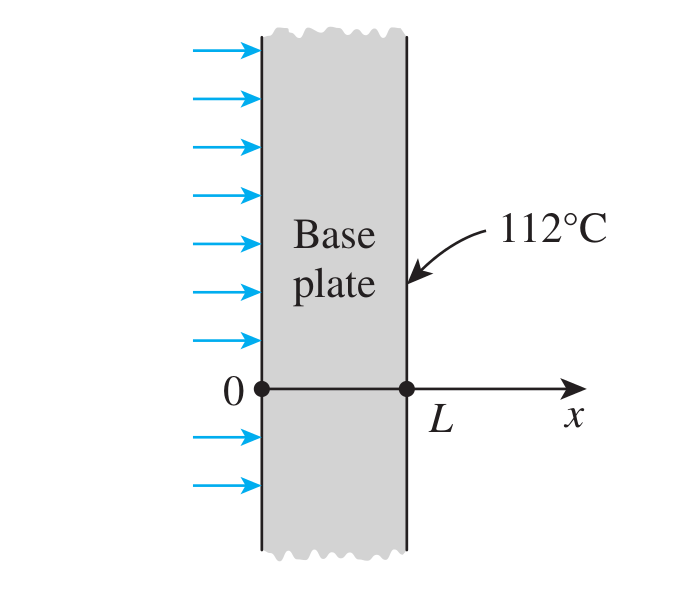
\includegraphics[width = 0.6\linewidth]{./image/lista1/q4}
\end{figure}

\subsection{}

Dado o calor fornedido pela resistência do ferro $\dot{Q}$, as temperaturas na parede interna e na superfície da base do ferro $\sympy{T0}$ e $\sympy{Tf}$, a condutividade térmica no ferro $\sympy{k}$ Pela lei de Fourier da condução de calor temos:

\begin{equation}\label{eq:fourierlaw-cond}
\dot{Q}(x) = \sympy{Derivative(Q,t)} = \sympy{dQ}
\end{equation}

Isolando $\sympy{Derivative(T,x)}$:

$$\frac{\dot{Q}}{\sympy{k*A}} = \sympy{Derivative(T,x)}$$

\subsection{}

Assumindo $\dot{Q}$ constante ao longo de todo o ferro e resolvendo a equação diferencial temos

\begin{equation}\label{eq:q4.Temp}
T = -\left(\frac{\dot{Q}}{\sympy{k*A}}\right)x + \sympy{T0}
\end{equation}

Em $x = 0$, temos $\dot{Q}(0) = \npy{dQ}\ W$, em $x=L$ temos $T(x=L) = \sympy{Tf} = \npy{Tf}^\circ $ e a espessuara da placa $L=\npy{L}$. Logo, a partir da equação \ref{eq:q4.Temp}:

$$T(L) = -\left(\frac{\dot{Q}}{\sympy{k*A}}\right)L + \sympy{T0} = -\frac{\npy{dQ}\cdot \npy{L}}{\npy{k}\cdot \npy{A}} + \sympy{T0}$$
$$T(L) = \sympy{round(-(ndQ*nL)/(nk*nA),4) + T0}$$

Isolando $\sympy{T0}$ e substituindo o valor de $T(L)$:

$$\sympy{T0} = \sympy{round(ndQ/(nk*nA),4)*L + Tf} =  \sympy{round((ndQ/(nk*nA))*nL,4)} + \npy{Tf} \Rightarrow \sympy{T0} = \sympy{round((ndQ/(nk*nA))*nL + nTf,4)}$$

Substituindo o valor de $\sympy{T0}$ na equação \ref{eq:q4.Temp}, encontramos T(x):

\begin{equation}\label{eq:q4.Temp}
T(x) = \sympy{-m*x} + \npy{T0}
\end{equation}

\subsection{}

% Plot Grafico da temperatura

% q5 --------------------------------------------------------------------------
\section{}

Considerando uma espessura $L$ tal que $x=L$ e sabendo se que a temperatura $T(x) = 65x+25$ e que $T(x=L) = 38^\circ C$ temos que $L$ será dado por:

$$L = \frac{T(x=L) - 25}{65} = \frac{(38) - 25}{65} \Rightarrow L = \sympy{round((38-25)/65,3)}$$

% q6 --------------------------------------------------------------------------
\section{}
\begin{sympycode}
# Símbolos algébricos
t = Symbol('t') # Tempo
T = Symbol('T') # Temperatura
x = Symbol('x') # distãncia
L = Symbol('L') # Espessura Placa
A = Symbol('A') # Área da base
Q = Symbol('Q') # Calor total
h = Symbol('h') # coeficiente conveccao
k = Symbol('k') # Condutividade térmica
T0 = Symbol('T_0') # Temperatura parede interna
Ta = Symbol('T_amb') # Temperatura ambiente

# Valores numéricos
nL = 0.2/100 # m
nA = 0.08 # m"2s
nk = 60 # W/(m C)
nh = 15 # W/(m^2 C)
nT0 = 80 # graus C
nTa = 25 # graus C

# Modelo como resistência térmica
Rcond = L/(k*A)
Rconv = 1/(h*A)

# Cálculo por divisor de tensão
Tf = -(Ta-T0)*(Rconv/(Rconv+Rcond))
nTf = Tf.subs([(L,nL),(A,nA),(k,nk),(h,nh),(T0,nT0),(Ta,nTa)])
\end{sympycode}

Considerando $R_{cond} = \sympy{Rcond}$ e $R_{conv} = \sympy{Rconv}$ podemos modelar o sistema como duas resistências em série:

% Modelo aproximado por circuitos

A partir do modelo temos que o fluxo de calor $\dot{Q}$ é

$$\dot{Q} = \frac{\sympy{-Ta+T0}}{R_{cond} + R_{conv}}  = \sympy{-(Ta-T0)/(Rconv+Rcond)}$$

Logo, o valor de $T_f$ pode ser encontrado por $T_f = \dot{Q} R_{conv}$ e portanto:

$$T_f = \sympy{Tf} = \sympy{Tf.simplify()} = \npy{Tf}$$

$$T_f = \frac{\npy{k}(\npy{T0} - \npy{Ta})}{\npy{L}\cdot \npy{h} + \npy{k}}= \npy{Tf}$$

% q7 --------------------------------------------------------------------------
\section{}

\begin{sympycode}
# Símbolos algébricos
t = Symbol('t') # Tempo
T = Symbol('T') # Temperatura
x = Symbol('x') # distãncia
L = Symbol('L') # Espessura Placa
A = Symbol('A') # Área da base
Q = Symbol('Q') # Calor total
h = Symbol('h') # coeficiente conveccao
k = Symbol('k') # Condutividade térmica
T0 = Symbol('T_0') # Temperatura parede interna
Ta = Symbol('T_amb') # Temperatura ambiente
Tf = Symbol('T_f') # Temperatura ambiente
c = Symbol('delta')
E = Symbol('Epsilon')

# Valores numéricos
nL = 0.2/100 # m
nA = 0.08 # m"2s
nk = 60 # W/(m C)
nh = 15 # W/(m^2 C)
nT0 = 80 # graus C
nTa = 25 # graus C

# Modelo como resistência térmica
Rcond = L/(k*A)
Rconv = 1/(h*A)
Rrand = 1/(E*c*A*(Tf*Tf+Ta*Ta)*(Tf+Ta))

Reqv =  Rcond + Rconv*Rrand/((Rconv+Rrand).simplify())

dQ2 = (Ta - Tf)/(Rconv*Rrand/((Rconv+Rrand).simplify()))
dQ1 = (Tf - T0)/Rcond

# Cálculo por divisor de tensão
Tf = -(Ta-T0)*(Rconv/(Rconv+Rcond))
nTf = Tf.subs([(L,nL),(A,nA),(k,nk),(h,nh),(T0,nT0),(Ta,nTa)])
\end{sympycode}

Considerando $R_{cond} = \sympy{Rcond}$ , $R_{conv} = \sympy{Rconv}$ e $R_{rand} = \sympy{Rrand}$ podemos modelar o sistema como duas resistências em série:

% Modelo aproximado por circuitos

A partir do modelo temos que o fluxo de calor $\dot{Q}$ é
%% Tentativa 1
%$$\dot{Q} = \frac{\sympy{-Ta+T0}}{R_{eqv}} =\frac{\sympy{-Ta+T0}}{R_{cond} + \frac{R_{conv}R_{rand}}{R_{conv}+R_{rand}}}$$
%$$\dot{Q} = \sympy{-(Ta-T0)/(Reqv)}$$

%% Tentativa 2
%$$\dot{Q} = \sympy{dQ1} = \sympy{dQ2}$$

???????????
%% Dúvidas Nesta Questão

% q8 --------------------------------------------------------------------------
\section{}

\begin{sympycode}
# Símbolos algébricos
t = Symbol('t') # Tempo
T = Symbol('T') # Temperatura
x = Symbol('x') # distãncia
L = Symbol('L') # Espessura Placa
A = Symbol('A') # Área da base
Q = Symbol('Q') # Calor total
h = Symbol('h') # coeficiente conveccao
k = Symbol('k') # Condutividade térmica
T0 = Symbol('T_0') # Temperatura parede interna
Ta = Symbol('T_amb') # Temperatura ambiente

# Modelo como resistência térmica
Rcond = L/(k*A)
Rconv = 1/(h*A)

# Valores numéricos
nT0 = 300 # graus C
nTa = 100 # graus C
nZ = 8

nL_a = 1*1e-3 #
nA_a = 12*1e-3*nZ #
nk_a = 2 #
nRcond_a = Rcond.subs([(L,nL_a),(k,nk_a),(A,nA_a)])

nL_b = 5*1e-3 #
nA_b = 4*1e-3*nZ #
nk_b = 8 #
nRcond_b = Rcond.subs([(L,nL_b),(k,nk_b),(A,nA_b)])

nL_c = 5*1e-3 #
nA_c = 4*1e-3*nZ #
nk_c = 20 #
nRcond_c = Rcond.subs([(L,nL_c),(k,nk_c),(A,nA_c)])

nL_d = 10*1e-3 #
nA_d = 6*1e-3*nZ #
nk_d = 15 #
nRcond_d = Rcond.subs([(L,nL_d),(k,nk_d),(A,nA_d)])

nL_e = 10*1e-3 #
nA_e = 6*1e-3*nZ #
nk_e = 35 #
nRcond_e = Rcond.subs([(L,nL_e),(k,nk_e),(A,nA_e)])

nL_f = 6*1e-3 #
nA_f = 12*1e-3*nZ #
nk_f = nk_a #
nRcond_f = Rcond.subs([(L,nL_f),(k,nk_f),(A,nA_f)])
\end{sympycode}

\begin{figure}[H]
\centering
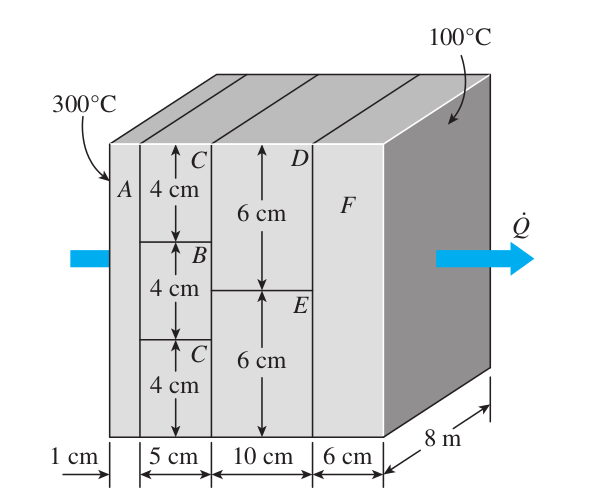
\includegraphics[width = 0.6\linewidth]{./image/lista1/q8}
\end{figure}

\subsection{}

Com base na equação \ref{eq:fourierlaw-cond} e a partir dos valores da condutância, espessura e área podemos calcular a resistência térmica para cada uma das partes do bloco. Desta forma obtemos os valores relacionados na tabela \ref{tab:q8.resistence}

\begin{table}[H]
\centering
\begin{tabular}{|cccc|c|}
\hline
 &  $L \ [m]$ &$A\ [m^2]$ & $k \ [W/m ^\circ C]$ & $R_{cond}$\\
\hline
A & \npy{L_a} & \npy{A_a} & \npy{k_a} & \npy{Rcond_a} \\
B & \npy{L_b} & \npy{A_b} & \npy{k_b} & \npy{Rcond_b} \\
C & \npy{L_c} & \npy{A_c} & \npy{k_c} & \npy{Rcond_c} \\
D & \npy{L_d} & \npy{A_d} & \npy{k_d} & \npy{Rcond_d} \\
E & \npy{L_e} & \npy{A_e} & \npy{k_e} & \npy{Rcond_e} \\
F & \npy{L_f} & \npy{A_f} & \npy{k_f} & \npy{Rcond_f} \\
\hline
\end{tabular}
\caption{Valores calculados para resistência térmica}
\label{tab:q8.resistence}
\end{table}

Desta forma podemos avaliar a resistência do bloco como associação das resistências para cada uma das partes conforme a figura \ref{fig:q8.circuit}

\begin{figure}[H]
    \centering
    \begin{circuitikz}[american voltages]
        \draw (0,0) to[R, l=$R_A$,*-*] (2,0);
        \draw (2,0) to (2,1);
        \draw (2,0) to (2,-1);
        \draw (2,1) to[R, l=$R_C$] (4,1);
        \draw (2,0) to[R, l=$R_B$] (4,0);
        \draw (2,-1) to[R, l=$R_C$] (4,-1);
        \draw (4,0) to (4,1);
        \draw (4,0) to (4,-1);
        \draw (4,0) to (5,0);
        \draw (5,0) to (5,0.5);
        \draw (5,0) to (5,-0.5);
        \draw (5,0.5) to[R, l=$R_D$] (7,0.5);
        \draw (5,-0.5) to[R, l=$R_E$] (7,-0.5);
        \draw (7,0) to (7,0.5);
        \draw (7,0) to (7,-0.5);
        \draw (7,0) to (7.5,0);
        \draw (7.5,0) to[R, l=$R_F$,*-*] (9.5,0);
    \end{circuitikz}
    \caption{Circuito Equivalente}
    \label{fig:q8.circuit}
\end{figure}

\begin{sympycode}
#
Ra = Symbol('R_A');
Rb = Symbol('R_B');
Rc = Symbol('R_C');
Rd = Symbol('R_D');
Re = Symbol('R_E');
Rf = Symbol('R_F');

R1 = (Rc/2)*Rb/((Rc/2)+Rb);
nR1 = R1.subs([(Rb,nRcond_b),(Rc,nRcond_c)]);
R2 = (Rd*Re)/(Rd+Re);
nR2 = R2.subs([(Rd,nRcond_d),(Re,nRcond_e)]);

Req1 = Ra+R1+R2+Rf;
nReq1 = Req1.subs([(Ra,nRcond_a),(Rb,nRcond_b),(Rc,nRcond_c),
   (Rd,nRcond_d),(Re,nRcond_e),(Rf,nRcond_f)])

nReq = (nReq1*(800/12))

nQ = (300 -100)/nReq;

nT3 = 300 - nQ*(nRcond_a+nR1)
\end{sympycode}

Definindo as resistências térmicas intermediárias $R_1$ e $R_2$, a partir das camadas formadas pelos materiais $C$, $D$ e $E$ temos:

$$R_1 = \sympy{R1} = \npy{R1}$$
$$R_2 = \sympy{R2} = \npy{R2}$$

Deste modo, podemos definir a resistência térmica do bloco da parede como:

$$R_{eq_1} = R_A + R_1 + R_2 + R_F$$
$$R_{eq_1} = R_A + \sympy{R1} + \sympy{R2} + R_F$$
$$R_{eq_1} = \npy{Req1}$$

Para parede toda a resistência será $R_{eq} = R_{eq_1}\cdot (800cm)/(12cm) = \npy{Req}$. Logo, a partir da resistência térmica podemos calcular a taxa de transferência de calor $\dot{Q}$, para as temperaturas $T_1 = 300^\circ C$ e $T_2 = 100^\circ C$ nas superficies da parede:

$$\dot{Q} = \frac{(T_1 - T_2)}{R_{eq}} = \frac{(300 - 100)}{\npy{Req}} = \npy{Q}\ W$$

\subsection{}

Assumindo a taxa de transferência de calor constante ao longo do bloco, a temperatura no ponto em que as seções B, D e E se encontram pode ser calculada como:
$$
T_3 = T_1 - \dot{Q}(R_A + R_1) $$
$$T_3= 300 - \npy{Q}\cdot ( \npy{Rcond_a} + \npy{R1}) = \npy{T3} ^\circ C
$$

\subsection{}
De maneira similar, a queda de temperatura ao longo do bloco $F$ pode ser calculada como
$$
\Delta T_f =  \dot{Q}\cdot R_F = \npy{Q}\cdot \npy{Rcond_f} = \npy{Q*nRcond_f} ^\circ C
$$

\section{} % q9
\paragraph{}Ao modelar a troca de calor por meio de resistências elétricas, a convecção e a radiação são modelas como resistências em paralelo devido representarem as trocas ocorridas da superfície externa com o meio.

\section{} % q10

\begin{figure}[H]
\centering
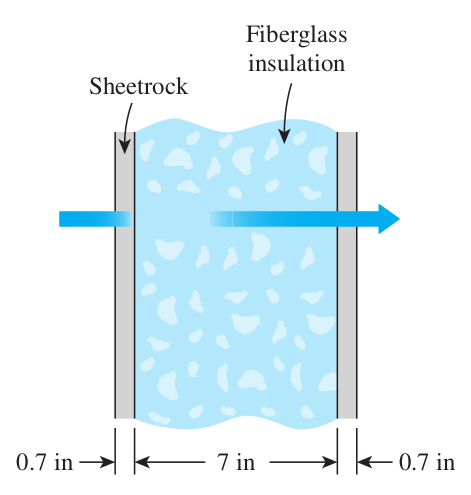
\includegraphics[width = 0.6\linewidth]{./image/lista1/q10}
\end{figure}

\begin{figure}[H]
    \centering
    \begin{circuitikz}[american voltages]
        \draw (0,0) to[R, l=$R_S$,*-*] (2,0);
        \draw (2,0) to[R, l=$R_F$,*-*] (4,0);
        \draw (4,0) to[R, l=$R_S$,*-*] (6,0);
    \end{circuitikz}
    \caption{Circuito Equivalente}
    \label{fig:q10.circuit}
\end{figure}



\section{} % q11

\begin{figure}[H]
\centering
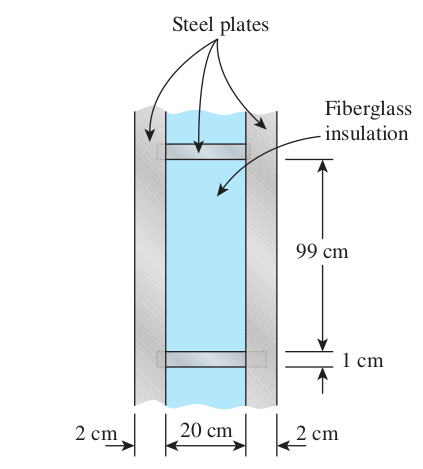
\includegraphics[width = 0.6\linewidth]{./image/lista1/q11}
\end{figure}

\section{} % q12

\section{} % q13

\begin{figure}[H]
\centering
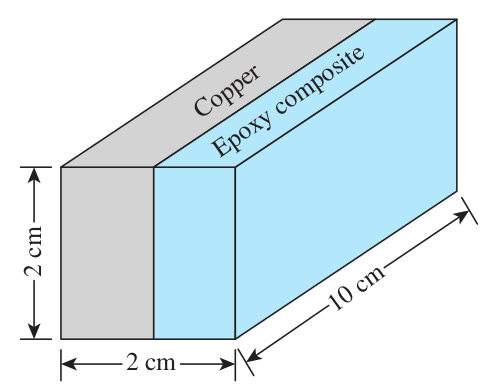
\includegraphics[width = 0.6\linewidth]{./image/lista1/q13}
\end{figure}

\section{} % q14

\section{} % q15

\begin{figure}[H]
\centering
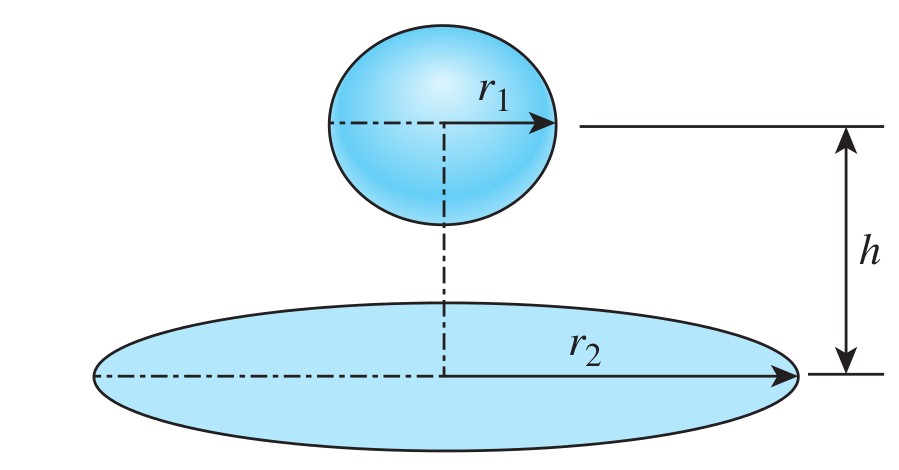
\includegraphics[width = 0.6\linewidth]{./image/lista1/q15}
\end{figure}

% ----------------------------------------------------------------------------
\end{document}
